\documentclass[../../templates/section]{subfiles}

\begin{document}

\section{Introduction}\label{sec:introduction}

Before we can begin to talk about what analysis is about, we must have a clear
notion of the objects that we want to study. Mathematics started with the study
of numbers and that's what we shall start with here. Just like driving a car
does not require knowledge of how an engine works, we will not enter into a
discussion of all properties of numbers(an interested reader might look to
\todo{more rigorous definition of numbers reference} for more information). We
must take some things for granted if we wish to get off the runway. We will
assume you to be familiar with rational, or decimal numbers such as
\begin{equation}\label{eq:numbers}
1, \qquad 2.56, \qquad \frac{1}{3}, \qquad 0.347
\end{equation}

This set of numbers is great for many purposes, including almost everything in
our day to day life, but we can show it isn't quite satisfactory for all
purposes. Take, for example, the following triangle.

\begin{figure}\label{fig:right-triangle}
    \centering
    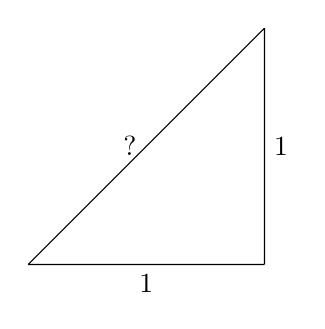
\begin{tikzpicture}
    \draw (0,0)  -- (3,0) node[midway, below]{1}
        (3,0) -- (3,3) node[midway, right]{1}
        (3,3) -- (0,0) node[midway, left]{?};
    \end{tikzpicture}
    \caption{Simple Right Triangle with Side Length 1}
\end{figure}

Suppose we want to figure out how long the side is labeled by ``?''. Well, if
we use the Pythagorean Theorem\footnote{This simply says that if we have a
right triangle with sides of length $a$ and $b$, then the hypotenuse $c$ is
related to those numbers by $c^2 = a^2 + b^2$.} then we can write the following
equation. We use the letter $x$ to denote the length of the hypotenuse that we
are interested in. 

\begin{align}
    x^2 & = 1^2 + 1^2 \nonumber \\ 
        & = 2         \nonumber \\ 
    x   & = \sqrt{2}  \label{eq:sqrt2}
\end{align}

If the rational numbers are ``enough''\footnote{meaning they represent
everything we can construct geometrically}, then we should be able to write $x$
as $\frac{n}{m}$ where $n$ and $m$ are integers ({$\{\ldots, -2, -1,
0, 1, 2, \ldots\}$})\todo{say rational numbers are fractions before this part}.
However, as we will see in \cref{ex:gaps}, this may not be the case.

\begin{example}[Existence of Gaps]\label{ex:gaps}
In this example we will set out to show that \cref{eq:sqrt2} has no
solutions that are rational. To show this we will employ a method known as
proof by contradiction. We will assume that $x$ can be written as a fraction
and try to arrive a contradiction.
\begin{equation}\label{eq:sqrt2-is-rational}
    x = \frac{n}{m}
\end{equation}
We take the fraction to be as reduced as possible\footnote{meaning we
wouldn't have something like $\frac{5}{15}$ because that can be reduced further
to $\frac{1}{3}$} and hence $n$ and $m$ are \emph{not both} even. If we plug
\cref{eq:sqrt2-is-rational} into \cref{eq:sqrt2} and square both sides we
obtain the following equation.
\begin{equation}
    \frac{n^2}{m^2} = 2
\end{equation}
We can then muliply both sides by $m^2$ to clear the denominator on the left
hand side and obtain
\begin{equation}\label{eq:oddeven}
    n^2 = 2m^2.
\end{equation}
Now here we make an important observation; $n^2$ is $2$ times another number.
What exactly does that tell us though? Well, if $a$ is two times $b$ ($a =
2b$), then we know that $a$ is even!\footnote{if $a$ and $b$ are both Integers}
Thus, we can conclude that $n^2$ is also even. With that knowledge, what can we
say about $n$? Well lets break it down by cases of $n$ being even or odd.
\begin{multicols}{2}
Take $n$ to be \textbf{even}. Then we can write $n = 2k$ where $k$ is a natural
number. If we square both sides we obtain $n^2 = 4k^2$, so $n^2$ would actually
be even which aligns with what we have found above.
\vfill\null
\columnbreak
Take $n$ to be \textbf{odd}. Any odd number can be written as $n = 2p + 1$
where $p$ is a natural number. If we square both sides we obtain $n^2 = 4k^2 +
4k + 1 = 2(2k^2 + 2k) + 1$ which is an odd number which we know $n^2$ is not.
\end{multicols}
Since we know that $n^2$ is even, we can conclude that $n$ must also be even,
because if it were odd, then $n^2$ would also be odd.

Now we know $n = 2k$ and we can go ahead and plug that into \cref{eq:oddeven}
to obtain
\begin{align}
    4k^2 & = 2m^2 \nonumber \\
    2k^2 & = m^2. \label{eq:m-is-even}
\end{align}
Well this looks oddly similar to \cref{eq:oddeven} except the two is on the
other side. Well as it turns out, using \emph{the same} argument we used to
show $n$ was even applies here to show $m$ is even as well.

So does this mean anything? Well from the outset, we made the important
assumption that the fraction $\frac{n}{m}$ was completely
reduced\footnote{which would imply that $n$ and $m$ cannot \emph{both} be
even}. Thus we haved arrived at a contradiction from our fundamental
assumptions and we can thus conclude that the number $\sqrt{2}$ is \textbf{not}
representable as a simple fraction.
\end{example}

We can study \cref{ex:gaps} in more detail if we split the rational numbers up
in the following way.\todo{position the following figure better}
\begin{figure}[!htb]
    \centering
    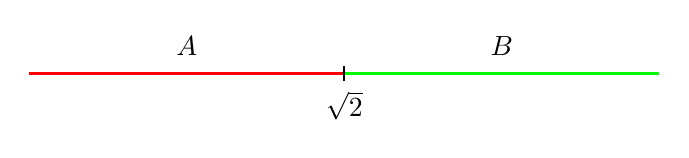
\begin{tikzpicture}[xscale=8]
    \draw[-][draw=red, very thick] (0,0) -- (.5,0);
    \draw[-][draw=green, very thick]  (.5,0) -- (1,0);
    \node[above] at (0.25, 0.1) {$A$};
    \node[above] at (0.75, 0.1) {$B$};
    \draw [thick] (0.5,-.1) node[below]{$\sqrt{2}$} -- (0.5,0.1);
    \end{tikzpicture}
\caption{Splitting the rational numbers into two groups}
\label{fig:split-rationals}
\end{figure}
More specifically, $A$ is the set of all rational numbers that are strictly
less than $\sqrt{2}$. Similarly, $B$ is the set of all rational numbers that
are strictly greater than $\sqrt{2}$.



\end{document}
